\subsection{Панель. Рабочий стол. Меню. Справка}

\subparagraph{1) Что нужно было сделать?}

Изучите информацию о панелях, рабочем столе, меню используемой вами системы в Справочной системе вашего дистрибутива.

\subparagraph{2) Как это сделали?}

Панель и мекю XFCE
на~рисунке~\ref{fig:mintwelcome}
(стр.~\pageref{fig:mintwelcome}).

\begin{figure}[!htp]
    \centering
    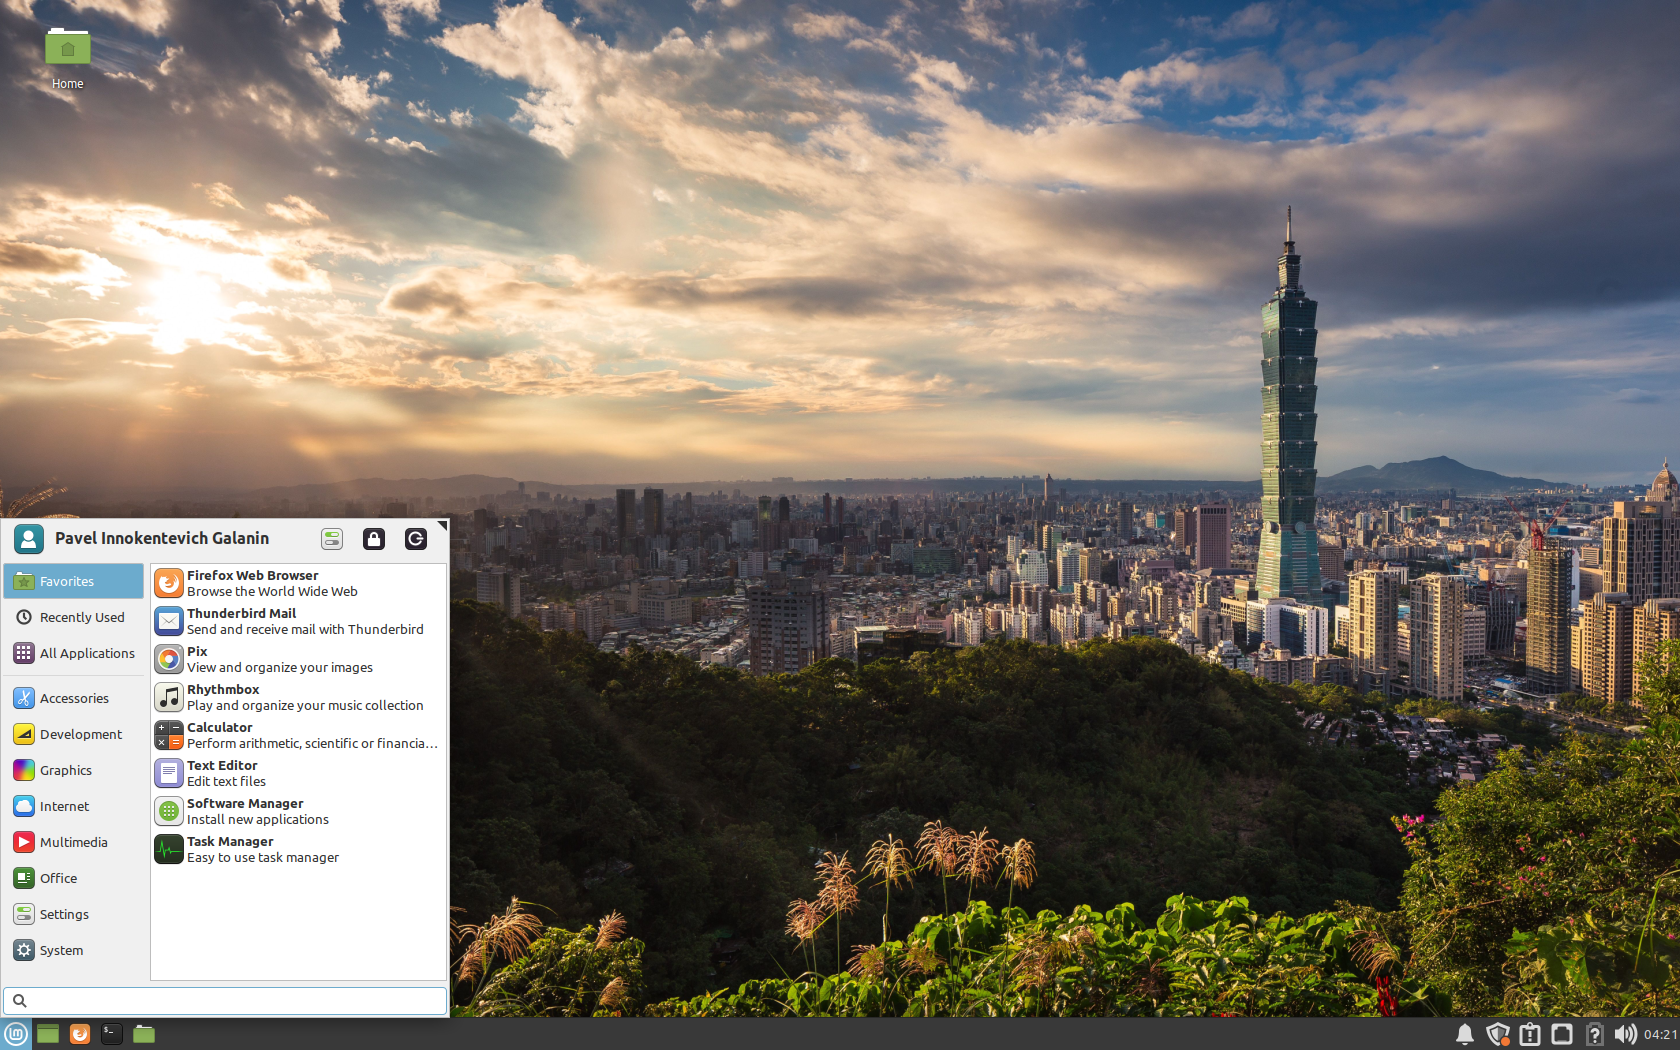
\includegraphics[width=11cm]
        {../input/task-2/1/menu.png}
    \caption{Панель и меню}
    \label{fig:panel}
\end{figure}

\begin{MyVerbatimCode}[label=Debian terminal]
pavel-innokentevich-galanin@aspire-one-725:~$ screenfetch
\end{MyVerbatimCode}

Результат команды
на~рисунке~\ref{fig:mintwelcome}
(стр.~\pageref{fig:mintwelcome}).

\begin{figure}[!htp]
    \centering
    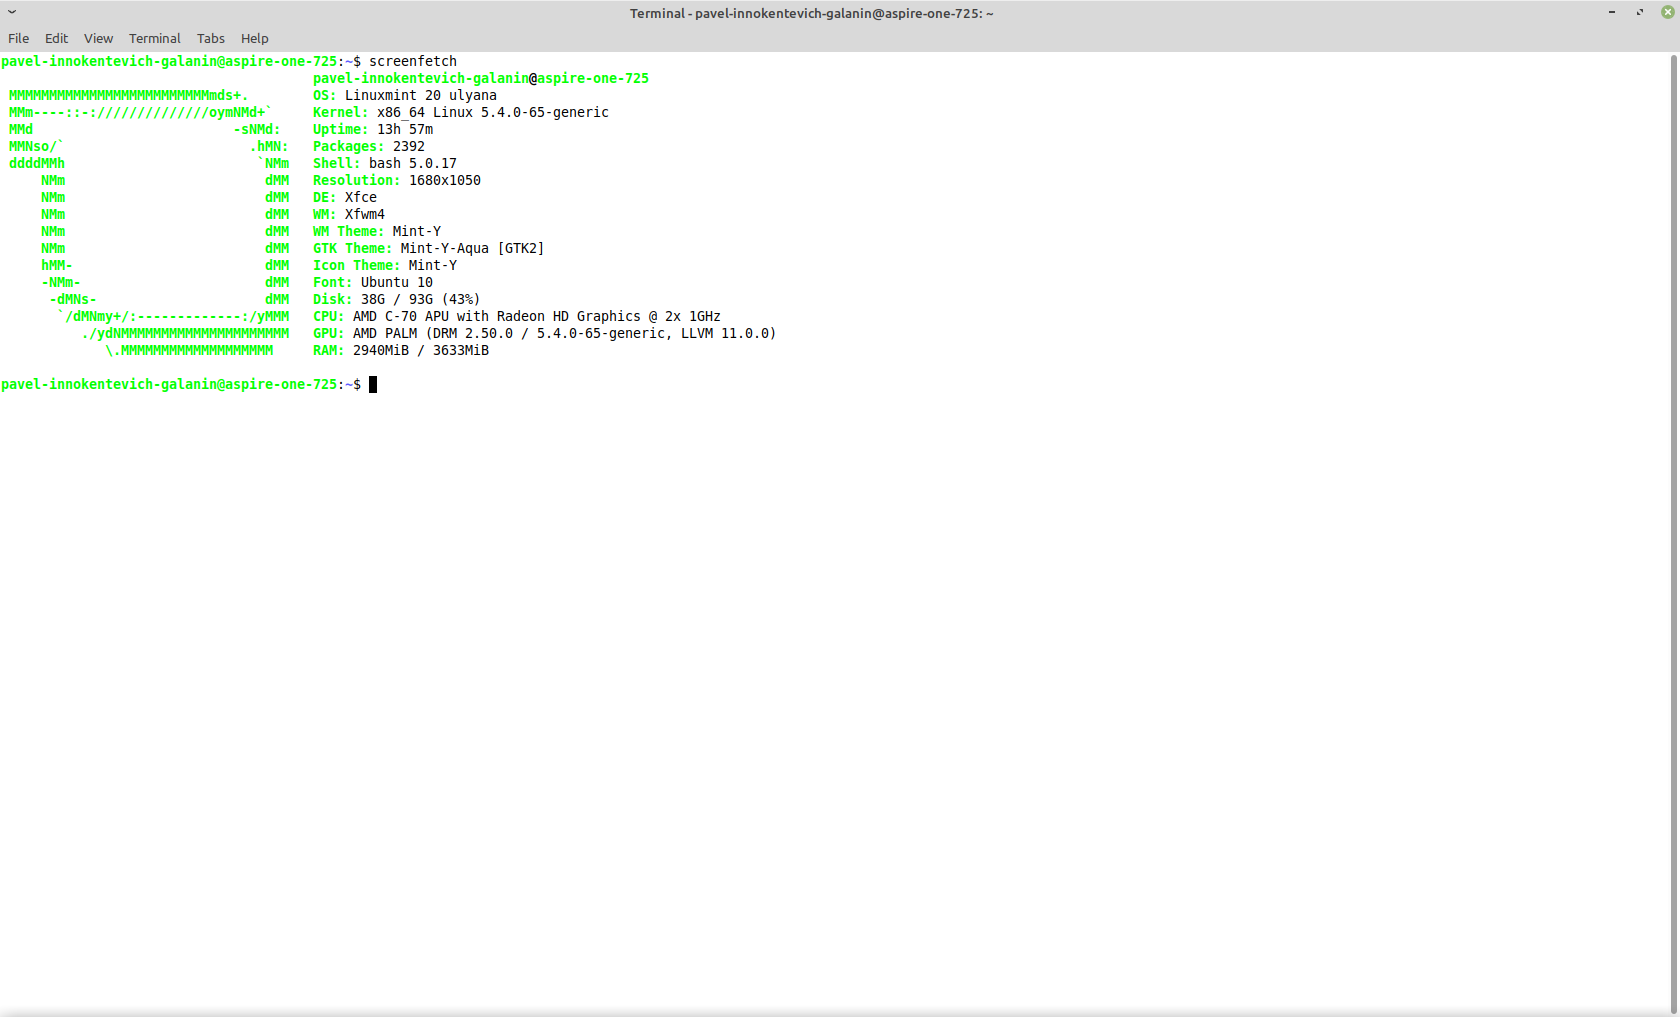
\includegraphics[width=11cm]
        {../input/task-2/1/screenfetch.png}
    \caption{screenfetch}
    \label{fig:screenfetch}
\end{figure}

Операционная система: Linuxmint 20 ulyana.

DE - Desktop Environment - окружение рабочего столя: Xfce.

\begin{MyVerbatimCode}[label=Debian terminal]
pavel-innokentevich-galanin@aspire-one-725:~$ mintwelcome
\end{MyVerbatimCode}

Скриншот Mint Welcome
на~рисунке~\ref{fig:mintwelcome}
(стр.~\pageref{fig:mintwelcome}).

Открытая документация в браузере
на~рисунке~\ref{fig:site-doc}
(стр.~\pageref{fig:site-doc}).

\begin{figure}[!htp]
    \centering
    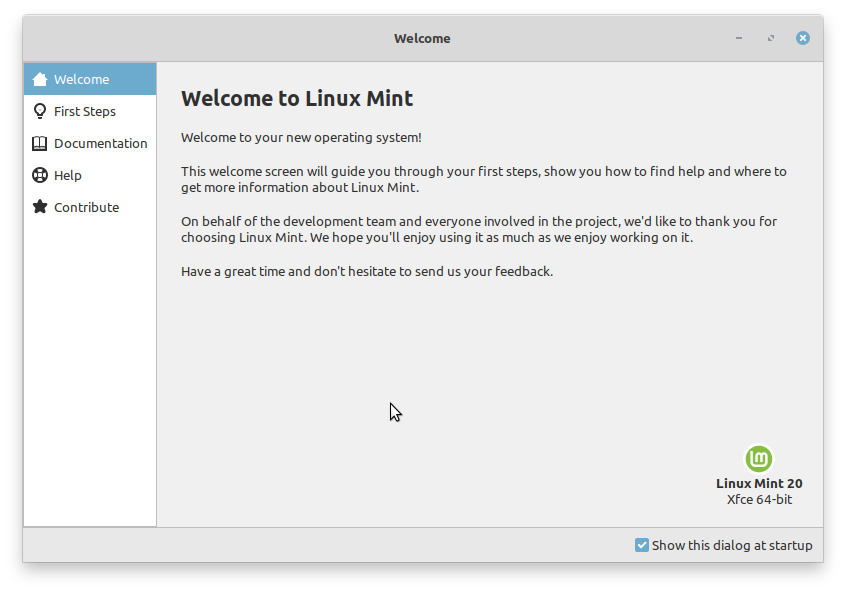
\includegraphics[width=11cm]
    {../input/task-2/1/mintwelcome.png}
    \caption{mint welcome}
    \label{fig:mintwelcome}
\end{figure}

\begin{figure}[!htp]
    \centering
    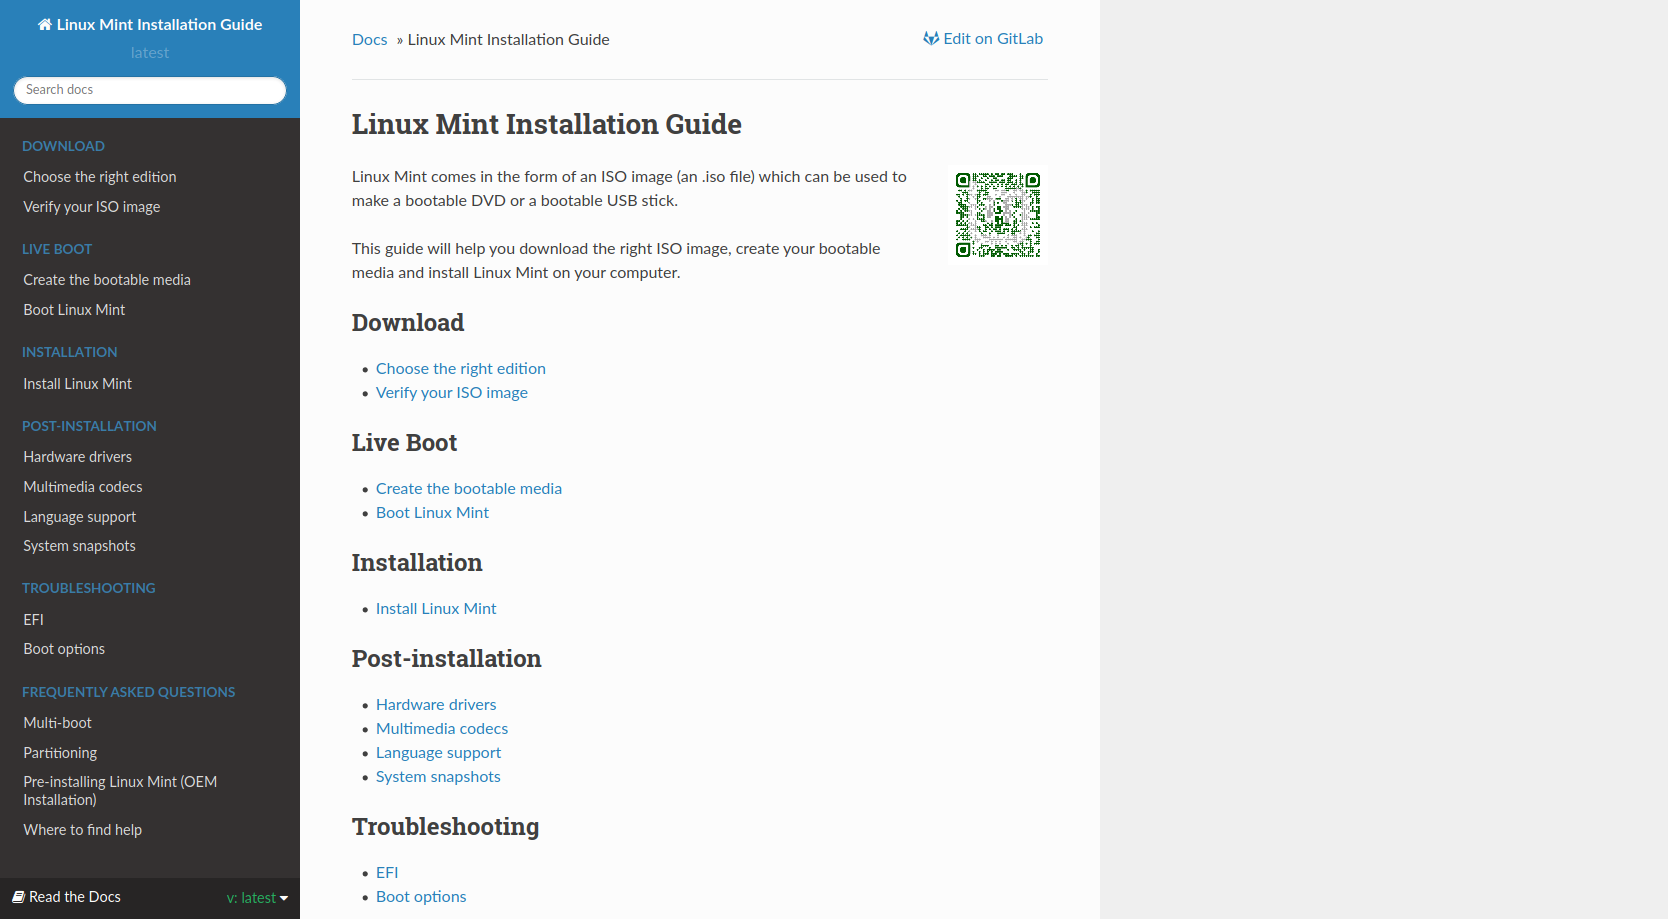
\includegraphics[width=11cm]
        {../input/task-2/1/site.png}
        \caption{Открытая документация в браузере}
        \label{fig:site-doc}
\end{figure}

\subparagraph{3) Что получилось?}

Посмотрели на панель и меню. Открыли приложение привествия. Почитали документацию.
